\section{Einleitung}
In diesem Kapitel wird zunächst vorgestellt, mit welchen Geräten der Fußschalter interagiert und die zusammen die \ac{HCT}-Plattform bilden. Es wird gezeigt, wie sich der Fußschalter in diese Plattform einfügt, sowie Motivation der Implementierung erklärt.

\subsection{HCT-Plattform}
Die Digitalisierung von Werkzeug in der Industrie ist in vollem Gange. Der Hauptgrund dafür ist, neben der einfacheren und genaueren Bedienung, die Möglichkeit durchgeführte Arbeitsschritte auf einem Computer automatisiert zu protokollieren. Wurden früher Messergebnisse per Hand vom Werkzeug auf Papier übertragen, werden sie nun zuverlässig und fehlerfrei mit Bluetooth an einen Computer übertragen. Das steigert die Effizienz und ermöglicht die Automatisierung der Qualitätskontrolle, sowie den Nachweis, dass Standards in der Fertigung eingehalten wurden, was in Branchen wie der Automobilindustrie oder der Luftfahrt von großer Bedeutung ist. \\
Dabei wurde sich für \ac{BLE} enschieden, da den Hand- und Messwerkzeugen, aufgrund ihrer handlichkeit und nicht kabelgebundenheit, nur begrenzte Batteriespeicherkapazitäten zu Verfügung stehen. \ac{BLE} ist eine Abwandlung des klassischen Bluetooth und ist besonders auf Energiesparkeit hin optimiert, wodurch es auch auf dem Hand- und Messwerkzeug lange Batterielaufzeiten garantieren kann.\\
Um die Digitalisierung der Messergebnisse dem Anwender so einfach wie möglich zu gestalten, setzt die Hoffmann Group mit der HCT-Plattform darauf, die Digitalisierung der durchgeführten Arbeitsschritte als einen festen Bestandteil in ihr Werkzeug zu integrieren. Diese sind zum Stand dieser Arbeit: 
\begin{itemize}
	\item Drehmomentschlüssel
	\item Messschieber bzw. Messuhren
	\item Drehmomentprüfgerät
\end{itemize}
Sie stellen dem Anwender die Daten der Messungen in verschiedener Weise zu Verfügung. Zum Einen können die Geräte als ein \ac{HID} über \ac{BLE} mit dem Computer verbunden werden. Sie simulieren dann eine über Bluetooth verbundene Tastatur über die, die Messergebnisse als Tastendrücke serialisiert werden. Das Messergebnis kann dann in einem Texteditor oder Excel aufgefangen werden. Des weiteren erzeugen die Drehmomentschlüssel und das Drehmomentprüfgerät eine \ac{CSV}-Datei, in der alle durchgeführten Messungen mit einer großen Anzahl an zusätzlichen Daten gespeichert werden. Wird das Gerät über \ac{USB} mit dem Computer verbunden, zeigt es sich als \ac{MSC}-Device und die Datei kann per Drag-and-drop auf den Computer kopiert werden. Die letzte Möglichkeit die durchgeführten Messungen zu digitalisieren, ist mithilfe der \ac{HCT}-Windows-App. Diese erfordert zusätzlich zur frei verfügbaren Software einen speziellen Dongle der zum Verbinden der Geräte benötigt wird. Sie werden ebenfalls über \ac{BLE} verbunden und sprechen über \ac{BLE} das firmeneigene \ac{HCT}-Protokoll. Die Windows-App bietet zahlreiche Möglichkeiten die Messdaten zu digitalisieren und den Produktionsprozess zu optimieren. Es können Schraubfälle in der App angelegt werden und mit Bildern hinterlegt werden. Die Seriennummer von Werkstücken kann automatisch mit dem dazugehörigen Messwert verlinkt werden und \ac{CAQ}-Software kann über einen virtuelle COM-Port angebunden werden. Die \ac{HCT}-Windows-App unterstützt derzeit lediglich die Drehmomentschlüssel, jedoch ist die Einbindung der restlichen \ac{HCT}-Geräte in Entwicklung. Der letzte Baustein der \ac{HCT}-Plattform ist die \ac{HCT}-Mobile-App, sie ist ebenfalls frei erhältlich und erleichtert vorallem die Bedienung des Geräts, zum Beispiel bei Arbeitsschritten bei denen das Display des Werkzeugs für den Anwender nicht sichtbar ist.

\subsection{HCT-Protokoll}
Der \ac{HCT}-Plattform liegt das firmeneigene \ac{HCT}-Protokoll zugrunde. Es stellt sicher, dass alle Geräte der \ac{HCT}-Plattform stets kompatibel zu einander sind. Es ist ein binäres Protokoll, dass entwickelt wurde um über \ac{BLE} gesprochen zu werden und stellt ein virtuelles Speichermodel der Geräte da. Dabei besitzten Werkzeuge unterschiedlicher Produktreihen und Hersteller jeweils verschiedene Speichermodelle. Über ``read'' und ``write'' Befehle auf die Speicheradressen kann dann der interne Zustand des Werkzeug abgefragt und verändert werden. So können auch komplexe Operationen effizient über \ac{BLE} durchgeführt werden. Zudem stehen automatisierte Tools zur Verfügung mit deren Hilfe die Frameworks, die das Sprechen des HCT-Protokoll abstrahieren, um die Speichermodelle neu eingeführter Werkzeuge erweitert werden kann.
\begin{figure}[H] 
	\centering
	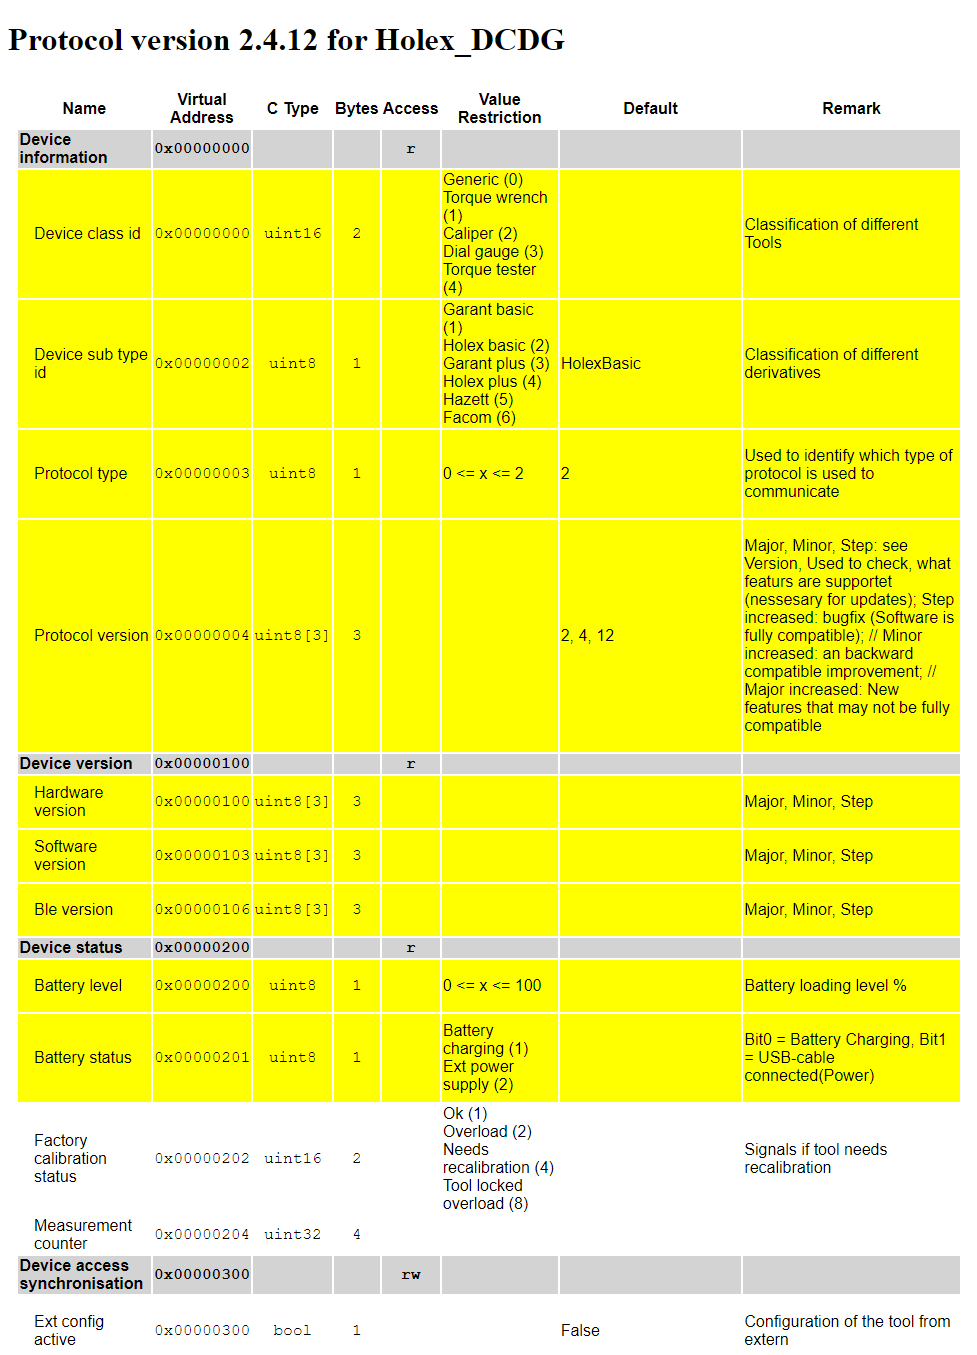
\includegraphics[width=\textwidth]{figures/HCT_Protocol_DCDG.png}
	\caption{Auszug aus \ac{HCT}-Protokoll für Messuhren und Messschieber}
\end{figure}

\subsection{Motivation}
Es hat sich gezeigt, dass die Einführung der \ac{HCT}-Windows-App immer wieder auf großen Widerstand von IT-Abteilungen trifft. Diese haben Sicherheitsbedenken, da die App direkt in der Fertigung eingesetzt wird und es müssen daher langwierige interne Prozesse für die Einführung angestoßen werden. Der Fußschalter soll ohne einer Installation die Funktion der Windows-App, die Serialisierung von Messergebnisse über einen virtuelle COM-Port im MUX50 bzw. DMX16-Protokoll, zur Verfügung stellen. \\
Des weiteren muss zum Senden eines Messwerts an den Computer bei Messschiebern und Messuhren eine Taste gedrückt werden. Bei der Durchführung von hochpräzisen Messungen, die auf den hundertstel Millimeter genau sein müssen, verfälscht dieses Betätigen einer Taste auf dem Gerät jedoch bereits die Messung. Auch bei der Durchführung von möglichst zeitgleichen Messungen mit mehreren Messgeräten stellt das Drücken einer Taste zum Senden des Messwerts den Nutzer vor Pro\ac{BLE}me. Daher werden in der Industrie Fußschalter eingesetzt, die kabelgebunden sowohl an das Werkzeug als auch an den Computer, dieses Senden der Messung auslösen können. Durch die kabelgebundene Natur dieser Fußschalter ist jedoch deren Einsatzbereich reduziert, da es nicht gegeben ist, dass in den Fertigungshallen und Werkstätten, in denen die Fußschalter eingesetzt werden, sich ein Computer in nächster Nähe befindet. Durch die Entwicklung eines Fußschalters der sich über Bluetooth mit dem Messwerkzeug verbindet, wird der Einsatzbereich deutlich vergrößert und der Einsatz dem Anwender erleichtert.